\documentclass{beamer}
\usepackage{tikz}
\usepackage{graphicx}
\usepackage{multimedia}
\usepackage{pgfplots}
\usepackage{pgfplotstable}
\pgfplotsset{width=1.1\textwidth,height=7.5cm,compat=1.9}
\usepackage{filecontents}
\usetikzlibrary{shapes,arrows,positioning,calc}
\usetheme[sectionpage=none]{metropolis}
\setsansfont[
        BoldFont={Fira Sans SemiBold},
        ItalicFont={Fira Sans Italic},
        BoldItalicFont={Fira Sans Bold Italic}
]{Fira Sans Book}
\definecolor{mred}{rgb}{0.8, 0.2, 0.06}

\title{Supercontinents and Superplumes}
\subtitle{in the Precambrian}
\date{November 14, 2019}
\author{Arijit Chakraborty}
\institute{Indian Institute of Science Education and Research, Kolkata}

\begin{filecontents}{shale.dat}
Age     Total   Thickness
600	0.50	675
600	0.76	813
650	0.10	165
650	0.27	51
650	0.35	126
660	0.30	120
660	0.33	165
700	0.40	720
750	0.30	480
790	0.80	500
850	0.34	161
850	0.76	519
1000	0.15	158
1000	0.30	81
1000	0.55	554
1050	0.26	260
1250	0.33	396
1450	0.20	600
1600	0.25	75
1640	0.20	406
1690	0.50	600
1700	0.40	1008
1700	0.55	1540
1750	0.35	201
1790	0.50	500
1850	0.90	540
1875	0.80	160
1878	1.00	2025
1880	0.31	248
1880	0.50	800
1880	0.54	3700
1900	0.40	250
1900	0.58	394
1925	0.46	306
1930	0.54	544
1975	0.63	628
1975	0.73	600
1995	0.80	1993
2000	0.30	158
2000	0.50	495
2100	0.40	120
2100	0.60	665
2150	0.25	255
2350	0.10	350
2350	0.25	575
2460	0.50	435
2530	0.65	449
2630	0.90	648
2700	0.70	105
\end{filecontents}

\begin{document}
        \maketitle

        \section{Supercontinents}

        \begin{frame}
        \frametitle{Supercontinents}
        \begin{figure}
        \centering
                \tikzset{
                        block/.style = {draw, fill=white, rectangle, minimum height=1em, minimum width=3em}
                }
                \begin{tikzpicture}[auto, node distance=2cm,>=latex']
                        \node [block] (mantle) {Mantle upwelling};
                        \node [block, right=-0.5cm of mantle, yshift=1.3cm] (breakup) {Supercontinent breakup};
                        \node [block, below=3cm of breakup] (formation) {Supercontinent formation};
                        \node [block, below=0.5cm of mantle] (shielding) {Shielding};
                        \node [block, right=0.3cm of breakup, yshift=-0.7cm] (avalanche) {Slab avalanche};
                        \node [block, below=0.5cm of avalanche] (plume) {Plume bombardment};
                        \node [block, below=0.5cm of plume] (juvenile) {Juvenile crust};
                        \draw [->] (mantle) |- (breakup);
                        \draw [->] (breakup) -- (formation);
                        \draw [->] (formation) -| (shielding);
                        \draw [->] (shielding) -- (mantle);
                        \draw [->] (breakup) -| (avalanche);
                        \draw [->] (avalanche) -- (plume);
                        \draw [->] (plume) -- (juvenile);
                        \draw [->] (juvenile) |- (formation);
                \end{tikzpicture}
        \end{figure}

        A \alert{supercontinent} is the assembly of most or all of Earth's cratons to form a single large landmass.

        \end{frame}
        
        \section{Superplumes}
        
        \begin{frame}
        \frametitle{Superplumes}
        A \alert{mantle plume} is an upwelling of abnormally hot rock within the Earth's mantle.

        A \alert{superplume} event is a short lived mantle plume event during which several plumes rose to the base of lithosphere.
        \pause

        \begin{center}
        Short lived = less than $100$ million years
        \end{center}
        \end{frame}

        \section{Seafloor spreading}
        
        \begin{frame}
        \frametitle{Sealevels}
        \begin{figure}
        \begin{center}
                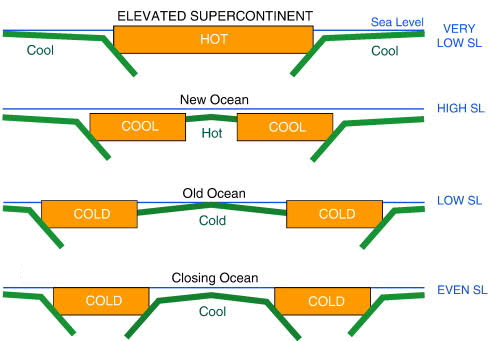
\includegraphics[width=0.75\textwidth]{seafloor.png}
        \end{center}
        \end{figure}
        \[
        \text{supercontinent} \;\implies\; \text{lots of old seafloor} \;\implies\; \text{low sea level}
        \]
        \end{frame}
        \begin{frame}
        \frametitle{Plate spreading}
        \begin{figure}[h!]
                \centering    
                \movie[externalviewer]{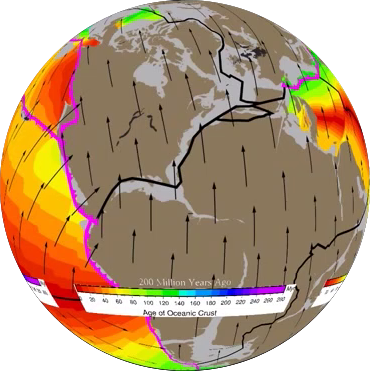
\includegraphics[width=5cm]{plate_movement.png}}{plate_movement.mp4}
        \end{figure}  

        Superplumes increase plate tectonic activity, hence the \emph{plate spreading} rate increases tremendously.
        \end{frame}
        
        \section{Superplumes - evidence}

        \begin{frame}
        \frametitle{Evidence for superplume events}
        \begin{itemize}
                \item Increase in \emph{surface temperature}.
                \item Deposition of black shale sediments with \emph{elevated $\delta^{13}C$} in sea water.
                \item Increased production of \emph{juvenile crust}.
                \item Rise in \emph{sea level}.
        \end{itemize}
        \end{frame}

        \begin{frame}
        \frametitle{Juvenile crust}
        \begin{figure}
        \begin{center}
                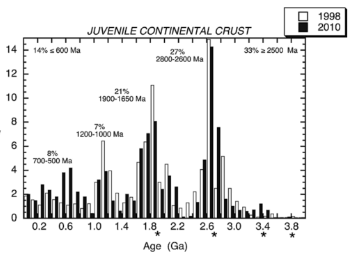
\includegraphics[width=0.9\textwidth]{juvenile.png}
        \end{center}
        \end{figure}
        \end{frame}
        
        \begin{frame}
        \frametitle{Supercontinent cycle \textit{vs} sealevel}
        \begin{figure}
        \begin{center}
                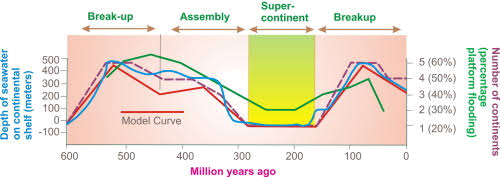
\includegraphics[width=\textwidth]{sealevel.png}
        \end{center}
        \end{figure}
        \end{frame}

        \section{Carbon}
        \begin{frame}
        \frametitle{Carbon reservoirs}
        \begin{center}
        \begin{tabular}{l | r}
                Pool    &       Quantity (gigatons) \\\hline\hline
                Atmosphere      &       720 \\
                Biosphere       &       2,000 \\
                Oceans          &       3,840 \\
                Fossil fuels    &       4,130 \\
                \alert{Lithosphere}     &       \alert{75,000,000}
        \end{tabular}
        \end{center}
        \end{frame}
        
        \begin{frame}
        \frametitle{Supercontinent cycle \textit{vs} carbon cycle}
                \begin{block}<1->{Supercontinent breakup}
                        \begin{itemize}
                                \item Tectonic plates get \emph{subducted} with lots of carbon deposits.
                                \item \emph{Volcanism} at mid-oceanic ridges releases $CO_2$.
                                \item Continental rift systems also release $CO_2$.
                        \end{itemize}
                \end{block}
                \begin{block}<2->{Supercontinent formation}
                        \begin{itemize}
                                \item \emph{Collision of plates} destroys rocks containing carbonates.
                                \item \emph{Surface area} of the supercontinent increases, hence weathering of rocks lowers $CO_2$ levels.
                        \end{itemize}
                \end{block}
        \end{frame}

        \begin{frame}
        \frametitle{Supercontinent cycle \textit{vs} carbon cycle}
        \begin{figure}
        \begin{center}
                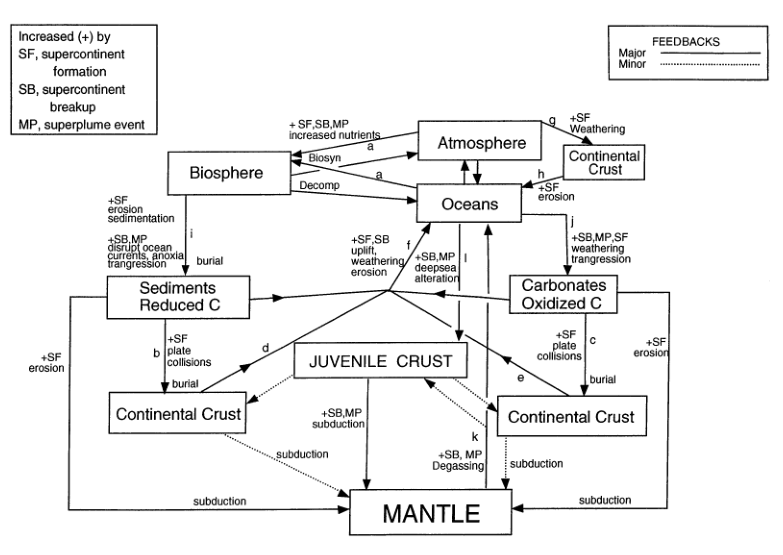
\includegraphics[width=\textwidth]{feedback.png}
        \end{center}
        \end{figure}
        \end{frame}

        \section{Black shale}

        \begin{frame}
        \frametitle{Black shale}
        \alert{Black shale} is a fine grained, sedimentary rock.
        
        It is formed in \emph{anoxic} and \emph{reducing} environments.
        
        \begin{figure}
        \begin{center}
                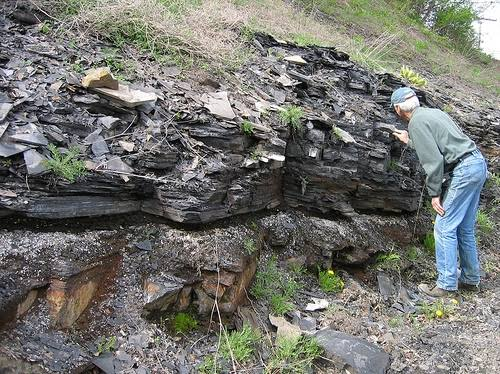
\includegraphics[width=0.7\textwidth]{shale_field.jpeg}
        \end{center}
        \end{figure}
        \end{frame}

        \begin{frame}
        \frametitle{Black shale deposits in the Precambrian}
        \begin{figure}
        \centering
        \begin{tikzpicture}
        \begin{axis}[
        axis y line=left,
        axis line style={draw=none},
        xtick={2800,2400,2000,1600,1200,800,400},
        ytick={0},
        ytick pos=left,
        yticklabels={,,},
        xlabel={Age (mya)},
        x tick style={rotate=90},
        x dir=reverse,
        ymin=0,ymax=6000,
        legend style={at={(0,0.4)},anchor=west},
        mlineplot
        ]
        \addplot+[samples y=0] table[x=Age,y=Thickness] {shale.dat};
        \addlegendentry{Thickness}
        \end{axis}
        \begin{axis}[
        axis y line*=right,
        axis line style={draw=none},
        xtick={2800,2400,2000,1600,1200,800,400},
        ytick={0},
        ytick pos=right,
        xticklabels={,,},
        yticklabels={,,},
        x dir=reverse,
        ymin=-2, ymax=1, 
        legend style={at={(0,0.45)},anchor=west},
        mlineplot
        ]
        \addplot+[samples y=0,mred,mark=square*,mark options={mred}] table[x=Age,y=Total] {shale.dat};
        \addlegendentry{Total amount}
        \end{axis}
        \end{tikzpicture}
        \end{figure}
        \end{frame}

        \begin{frame}
        \frametitle{$\delta^{13} C$ in black shale}
        \begin{figure}
        \begin{center}
                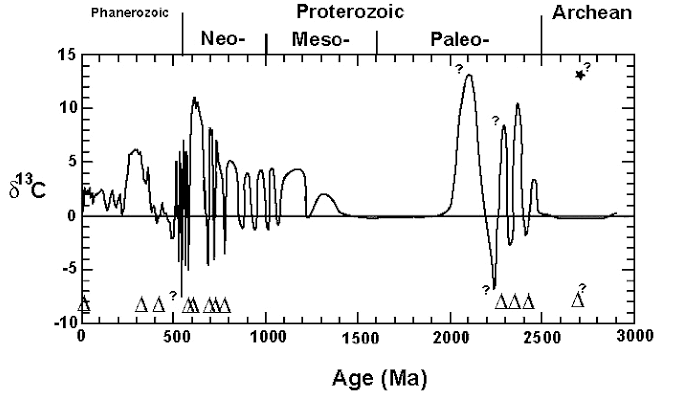
\includegraphics[width=\textwidth]{shale_carbon.png}
        \end{center}
        \end{figure}
        \end{frame}
        
        \begin{frame}[standout]
                Thank you!
                \pause

                Questions?
        \end{frame}
\end{document}
